 \begin{frame}{Functions}
  
    \begin{definition}
      Suppose that $X$ and $Y$ are sets.
      We say we have a function $f$ from $X$ to $Y$ if for each $x$ in $X$ we can specify a unique element in $Y$, which we denote by $f(x)$.
    \end{definition}
  
    \begin{center}
      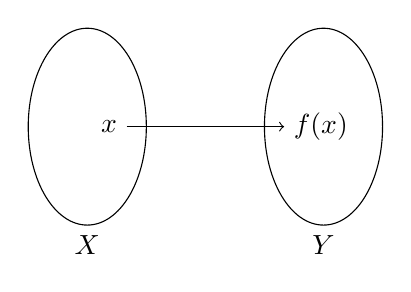
\begin{tikzpicture}
        \draw (0,0) ellipse (0.75 and 1.25);
        \draw (0,-1.5) node {$X$};
        \draw (3,0) ellipse (0.75 and 1.25);
        \draw (3,-1.5) node {$Y$};
  
        \draw [->]  (0.5,0) node[anchor=east] {$x$} -- (2.5,0) node[anchor=west] {$f(x)$};
      \end{tikzpicture}
    \end{center}
  
  \end{frame}
  
  
  
  \begin{frame}{Bijections}
  
    \begin{definition}
      A bijection is function $f$ from a set $X$ to a set $Y$ where both of the following are true:
        \begin{itemize}
          \item every $y$ in $Y$ is a value $f(x)$ for at most one $x$ in $X$.
          \item every $y$ in $Y$ is a value $f(x)$ for at least one $x$ in  $X$.
        \end{itemize}
    \end{definition}
  
    \begin{center}
      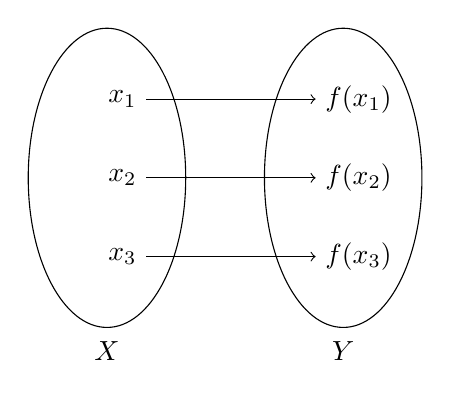
\begin{tikzpicture}
        \draw (0,0) ellipse (1 and 1.9);
        \draw (0,-2.2) node {$X$};
        \draw (3,0) ellipse (1 and 1.9);
        \draw (3,-2.2) node {$Y$};
  
        \draw [->]  (0.5,1) node[anchor=east] {$x_1$} -- (2.65,1) node[anchor=west] {$f(x_1)$};
        \draw [->]  (0.5,0) node[anchor=east] {$x_2$} -- (2.65,0) node[anchor=west] {$f(x_2)$};
        \draw [->]  (0.5,-1) node[anchor=east] {$x_3$} -- (2.65,-1) node[anchor=west] {$f(x_3)$};
      \end{tikzpicture}
    \end{center}
  
  \end{frame}
  
  
  \begin{frame}{Isomorphism}
  
    \begin{definition}
      Two graphs $G_1$ and $G_2$ are said to be isomorphic when there is a bijection $\alpha$ for the vertex set $V_1$ of $G_1$ to the vertex set $V_2$ of $G_2$ such that $\{\alpha (x) , \alpha (y) \}$ is an edge of $G_2$ if and only if $(x,y)$ is an edge of $G_1$.
    \end{definition}
      
    \begin{center}
      \begin{columns}
        \begin{column}{0.3\textwidth}
          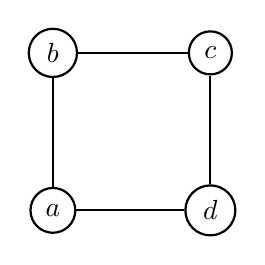
\begin{tikzpicture}
            \begin{scope}[every node/.style={circle,thick,draw}]
              \node (a) at (0,0) {$a$};
              \node (b) at (0,2) {$b$};
              \node (c) at (2,2) {$c$};
              \node (d) at (2,0) {$d$};
            \end{scope}
            \begin{scope}[every edge/.style={draw=black,thick}]
              \path (a) edge (b);
              \path (b) edge (c);
              \path (c) edge (d);
              \path (d) edge (a);
            \end{scope}
          \end{tikzpicture}
        \end{column}
        
        \begin{column}{0.3\textwidth}
          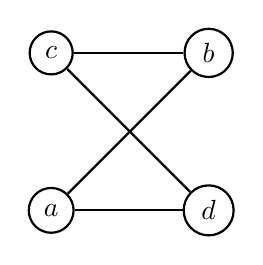
\begin{tikzpicture}
            \begin{scope}[every node/.style={circle,thick,draw}]
              \node (a) at (0,0) {$a$};
              \node (c) at (0,2) {$c$};
              \node (b) at (2,2) {$b$};
              \node (d) at (2,0) {$d$};
            \end{scope}
            \begin{scope}[every edge/.style={draw=black,thick}]
              \path (b) edge (c);
              \path (c) edge (d);
              \path (b) edge (a);
              \path (d) edge (a);
            \end{scope}
          \end{tikzpicture}
        \end{column}
        
        \begin{column}{0.3\textwidth}
          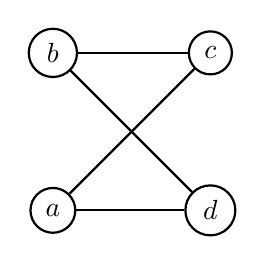
\begin{tikzpicture}
            \begin{scope}[every node/.style={circle,thick,draw}]
              \node (a) at (0,0) {$a$};
              \node (b) at (0,2) {$b$};
              \node (c) at (2,2) {$c$};
              \node (d) at (2,0) {$d$};
            \end{scope}
            \begin{scope}[every edge/.style={draw=black,thick}]
              \path (b) edge (c);
              \path (b) edge (d);
              \path (c) edge (a);
              \path (d) edge (a);
            \end{scope}
          \end{tikzpicture}
        \end{column}
      \end{columns}
    \end{center}
  
  \end{frame}
  
  
  \begin{frame}{Isomorphism example}
    \begin{center}
      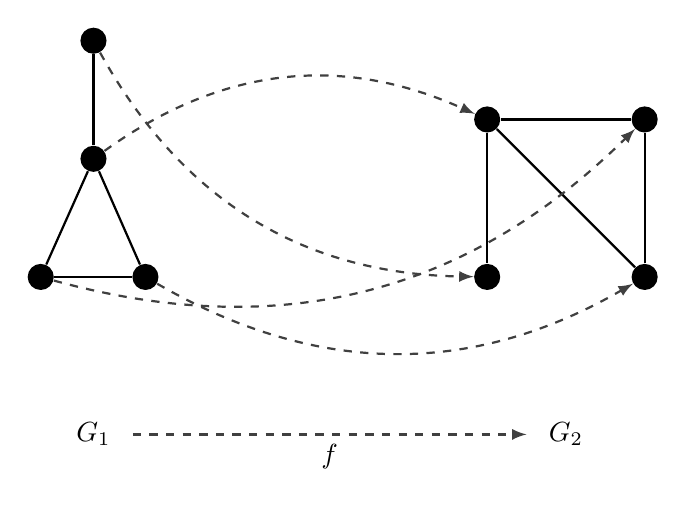
\begin{tikzpicture}
        \begin{scope}[every node/.style={circle, fill=black}]
          \node (a) at (1   ,1.5) {};
          \node (b) at (1   ,3) {};
          \node (c) at (0.33,0) {};
          \node (d) at (1.66,0) {};
        \end{scope}
        \begin{scope}[every edge/.style={draw=black,thick}]
          \path (a) edge (b);
          \path (a) edge (c);
          \path (a) edge (d);
          \path (c) edge (d);
        \end{scope}
        \begin{scope}[every node/.style={circle, fill=black}]
          \node (1) at (6,2) {};
          \node (2) at (6,0) {};
          \node (3) at (8,2) {};
          \node (4) at (8,0) {};
        \end{scope}
        \begin{scope}[every edge/.style={draw=black,thick}]
          \path (1) edge (2);
          \path (1) edge (3);
          \path (1) edge (4);
          \path (3) edge (4);
        \end{scope}
        \begin{scope}[every edge/.style={draw=darkgray, dashed, thick, ->, >=latex}]
          \path (a) edge[bend left] (1);
          \path (b) edge[bend right] (2);
          \path (c) edge[bend right] (3);
          \path (d) edge[bend right] (4);
        \end{scope}
        \node at (1,-2) {$G_1$};
        \node at (7,-2) {$G_2$};
        \path (1.5,-2) edge[draw=darkgray, dashed, thick, ->, >=latex] node[below] {$f$} (6.5,-2);
      \end{tikzpicture}
    \end{center}
  \end{frame}
  
  \begin{frame}{Isomorphism: degrees}
  
    \begin{block}{Exercise}
      Determine if these two graphs are isomorphic.
  
      \begin{columns}
        \begin{column}{0.5\textwidth}
          \begin{center}
            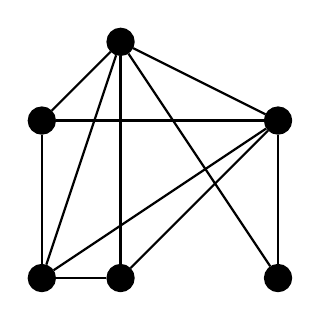
\begin{tikzpicture}
              \begin{scope}[every node/.style={circle,thick,draw,fill}]
                \node (a) at (0,1) {};
                \node (b) at (0,4) {};
                \node (c) at (2,1) {};
                \node (d) at (2,3) {};
                \node (e) at (-1,1) {};
                \node (f) at (-1,3) {};
              \end{scope}
              \begin{scope}[every edge/.style={draw=black,thick}]
                \path (a) edge (b);
                \path (a) edge (d);
                \path (a) edge (e);
                \path (b) edge (c);
                \path (b) edge (d);
                 \path (b) edge (e);
                 \path (b) edge (f);
                 \path (c) edge (d);
                 \path (d) edge (e);           
                 \path (d) edge (f);
                 \path (e) edge (f);
              \end{scope}
            \end{tikzpicture}
          \end{center}
        \end{column}
        \begin{column}{0.5\textwidth}
          \begin{center}
            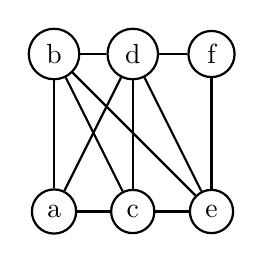
\begin{tikzpicture}
              \begin{scope}[every node/.style={circle,thick,draw}]
                \node (a) at (0,0) {a};
                \node (b) at (0,2) {b};
                \node (c) at (1,0) {c};
                \node (d) at (1,2) {d};
                \node (e) at (2,0) {e};
                \node (f) at (2,2) {f};
              \end{scope}
              \begin{scope}[every edge/.style={draw=black,thick}]
                \path (a) edge (b);
                \path (a) edge (c);
                \path (c) edge (e);
                \path (a) edge (d);
                \path (b) edge (c);
                \path (b) edge (d);
                 \path (b) edge (e);
                 \path (b) edge (d);
                 \path (d) edge (f);
                 \path (c) edge (d);
                 \path (d) edge (e);	            
                 \path (e) edge (f);
              \end{scope}
            \end{tikzpicture}
          \end{center}
        \end{column}
      \end{columns}
    \end{block}
  \end{frame}

\end{document}
 